\begin{figure}[!ht]
    \centering
    \vspace{0.2cm}
    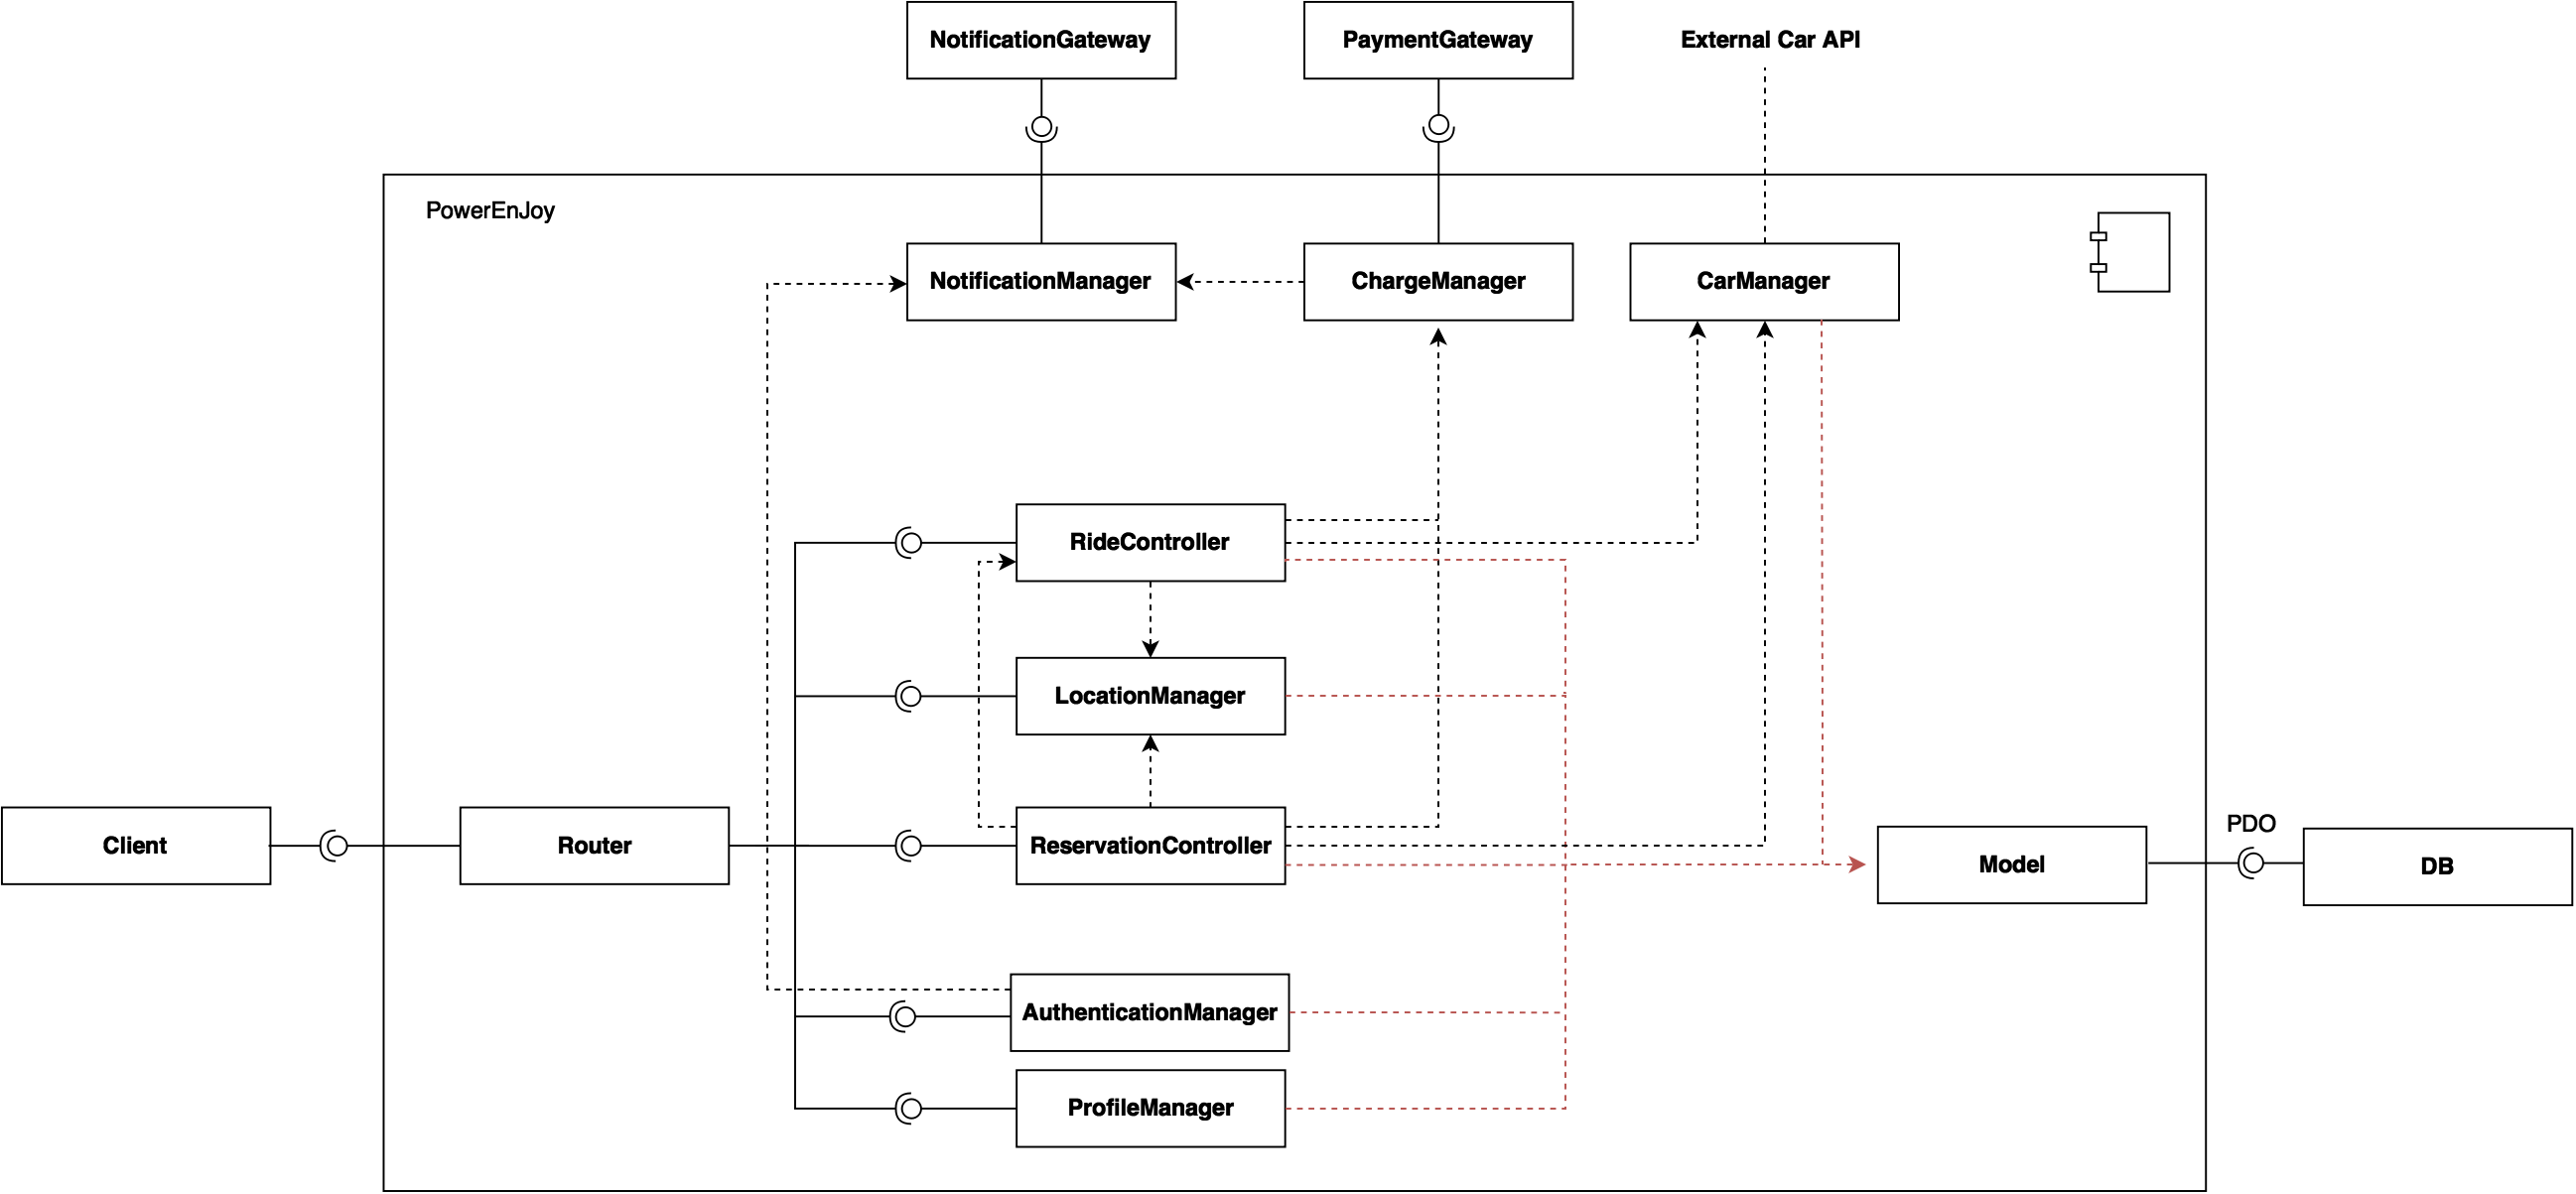
\includegraphics[width=1.0\textwidth]{/DD/component_view}\\
    \vspace{0.4cm}
    \caption{Component view for the Application Server} 
    \label{fig:component_view} 
\end{figure}

\subsection{System components}
To define and easily understand what kind of functionalities must be implemented in our system we decided to decompose PowerEnJoy logically into components, which are reusable and easily adaptable bricks for our application. 
\\In this section the single components and their interactions are analysed, the router component is not represented for sake of simplicity. 

\begin{itemize}
	\item \textbf{AuthenticationManager}: This component provides all the authentication-related functionalities such as registration, login, credentials generation and password recovery. It is important to remark here that a RESTful API is provided and so no session is created, instead a token is provided and used for authentication purposes.
	\item \textbf{ProfileManager}: This component manages all the profile-related functionalities in order to allow informations' editing.
	\item \textbf{LocationManager}: This component handles the logic behind the vehicle/user localization and tracking, it is also responsible for safe-areas and charging-stations' location consistency.
	\item \textbf{ReservationController}: This component manages the reservation logic, it receives informations from the LocationManager, correctly handles the timing for expiration and queries the CarManager component to update the car status (FREE, RESERVED, INUSE, OUTOFSERVICE). It is responsible for the Reservation logic and correctness checking.
	\item \textbf{RideController}: This component controls the (un)locking of the car, the car status and correctly handles the timing and charges for the ride. It is responsible for the Ride logic and correctness checking.
	\item \textbf{CarManager}: This component is responsible for communications with the on-board computer and for car's status update.
	\item \textbf{ChargeManager}: This component handles the application of charges for rides and reservations, it also process the applications of fees and discounts due to bad/virtuous behaviours. It is responsible to communicate with the PaymentGateway to complete the payment process.
	\item \textbf{NotificationManager}: This component manages the users' notification, in particular regarding charges and payment requests. It communicates with the NotificationGateway to effectively notify the users.
	\item \textbf{PaymentGateway}: This component is responsible for the communication with the external payment handler in order to effectively process the payments(automatic payments are pre-authorized).
	\item \textbf{NotificationGateway}: This component actually creates and send the user notification.
	\item \textbf{Router}: This component is responsible for routing the requests to the correct components.
	\item \textbf{Client}: The actual client device(Mobile/Web application).
	\item \textbf{Model}: The data we interact with, this is an abstraction of the DataBase.
	\item \textbf{DataBase}: The database used to store persistent data.
\end{itemize}

\newpage
\subsection{Database components}
The data stored in the database will be split into different subcomponents that identifies the main entities of our system:
User,Vehicle, Location, Safe Area, Charging Station, Reservation, Ride, Behaviours and Payment.  
\\The designed model for persistent data is provided here in a ER diagram in order to better analyze the motivations of our design. That's the representation of the database model:
\begin{figure}[!ht]
  \centering
  \vspace{0.2cm}
  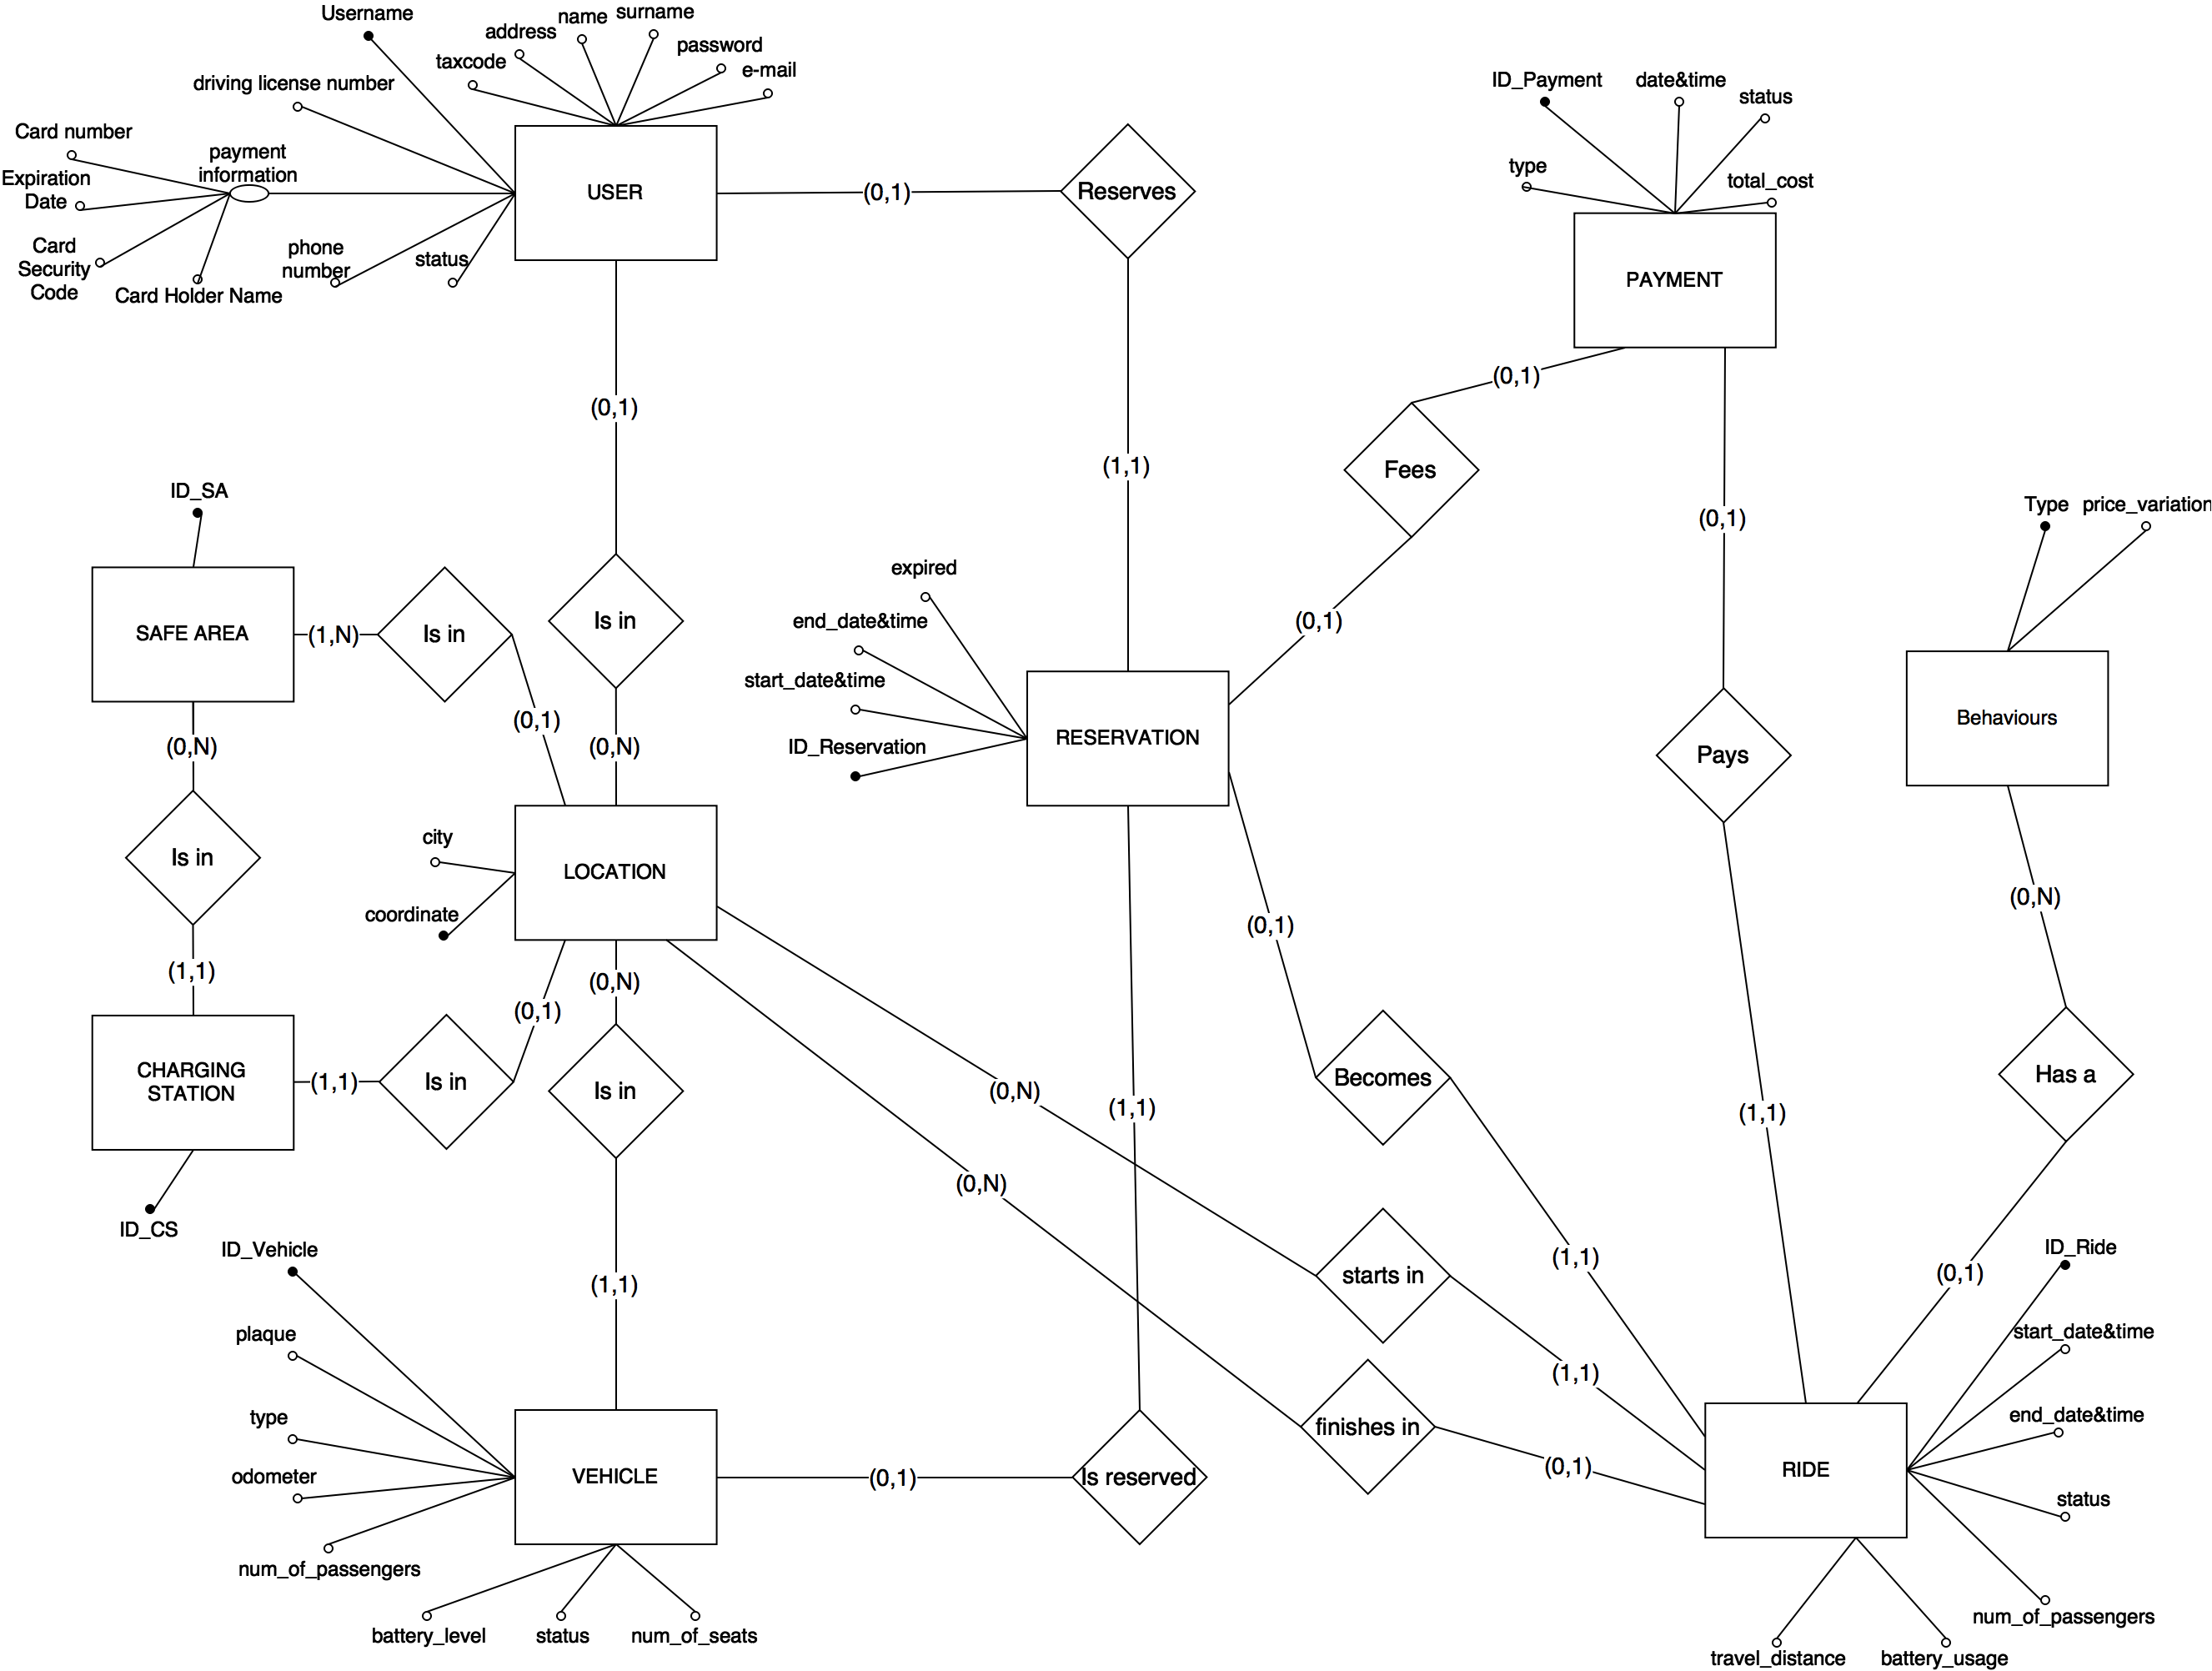
\includegraphics[width=1.0\textwidth]{/DD/ER_Diagram}\\
  \vspace{0.4cm}
  \caption{ER Diagram} 
  \label{fig:ER_Diagram} 
\end{figure}

 And this is the relation schema associated with the ER diagram.
\begin{itemize} 
	\item{User (\underline{taxcode}, \textit{Location}, e-mail, password, driving\_license\_number, name, surname, address, phone number, card\_number, expiration\_date, security\_code, locked)}
	\item{Vehicle (\underline{ID}, \textit{Location}, plate, type, odometer, battery\_level, status, num\_of\_seats, num\_of\_passengers) }
	\item{Location (\underline{ID}), longitude, latitude}	
	\item{Safa Area (\underline{ID}, \underline{Location})} %type A=Safe Area, B=Charging Station, C=both, Add an ID!!!
	\item{Charging Station(\underline{ID}, \textit{Location},\textit{ID\_SafeArea})}
	\item{Reservation (\underline{ID}, \textit{ID\_User}, \textit{ID\_Vehicle}, start\_date\&time, end\_date\&time, expired)}
	\item{Ride (\underline{ID}, \textit{ID\_User}, \textit{ID\_Vehicle}, \textit{ID\_Reservation}, \textit{ID\_Payment},\textit{Start\_Location},\textit{End\_Location}, start\_date\&time, end\_date\&time, num\_of\_passengers, travel\_distance, battery\_usage)}
	\item{Behaviours(\underline{Type}, \underline{\textit{ID\_Ride}}, price\_variation)}
	\item{Payment (\underline{ID}, \textit{ID\_User}, \textit{ID\_Reservation}, \textit{ID\_Ride}, date\&time, total\_cost, status, type)}
\end{itemize}
In the User entity there are all the main informations about the user such as credentials and payment method. User lock tag can be either TRUE or FALSE. The user's location is not mandatory.
\\A Vehicle entity has different attributes, some of them supplied by the On-Board computer. The status here can be FREE, RESERVED, INUSE or OUTOFSERVICE.
\\The Location entity represent a location provided by the GPS. Safe areas are zones composed by one or more locations disposed in poligons, which can contain Charging stations.
\\A reservation is associated with a Payment object if and only if it is expired. Reservations are strictly connected with the Ride entity, which can exist only related with it. Each ride has a starting point and when it finishes an end point. 
\\Every Ride is associated with a Payment object, in particular the presence of a related Behaviour object implies a variation of the final price. 
\\In the Payment entity there are informations about the transaction from the user to PowerEnJoy, the status indicates if the payments succeeded or is pending.
